\problemname{\problemyamlname}

%\illustration{0.3}{image.jpg}{Caption of the illustration (optional). CC BY-NC 2.0 by X on Y}
% Source: URL to image.

% optionally define variables/limits for this problem
En prévision de la prochaine édition du BAPC à l'UCLouvain, la société KARWa Corp. souhaite relier tous les karaokés de Belgique entre eux.
Pour cela, elle contacte la SNCB et la STIB qui font appel à vous pour trouver la meilleure façon de relier tous les karaokés.

Il y a $n$ karaokés numérotés de $1$ à $n$ et $m$ liaisons bidirectionnelles entre certains d'entre eux.
Chaque liaison a un poids $w$ représentant la distance entre les deux karaokés reliés.
L'objectif est de relier tous les karaokés entre eux tout en minimisant le coût (distance) total de toutes les liaisons.

Cependant, les petites liaisons (avec un petit poids) sont chères, la SNCB souhaite donc maximiser le poids de l'arête minimale de sorte que le coût (la distance) total des liaisons soit inférieur à $125\%$ du coût (de la distance) minimal pour relier tous les karaokés.
Autrement dit, le coût total des liaisons doit être inférieur ou égal à $1.25$ fois le coût minimum pour que le projet soit viable.

Il est garanti qu'il est possible de relier tous les karaokés entre eux.

\begin{figure}[h]
	\centering
	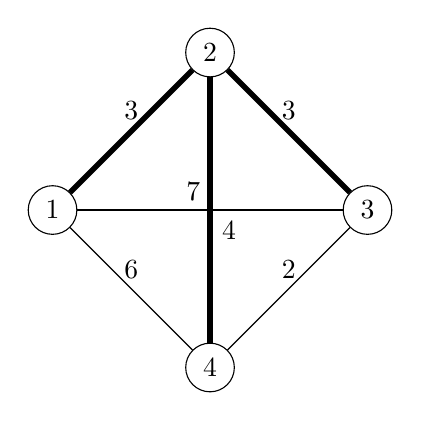
\begin{tikzpicture}
		% Définition des noeuds
		\node[circle,draw] (1) at (0,0) {1};
		\node[circle,draw] (2) at (2,2) {2};
		\node[circle,draw] (3) at (4,0) {3};
		\node[circle,draw] (4) at (2,-2) {4};
		
		% Définition des arêtes
		\draw (1) -- node[above]{6} (4);
		\draw[line width=2pt] (1) -- node[above]{3} (2);
		\draw[line width=2pt] (2) -- node[above]{3} (3);
		\draw (3) -- node[above]{2} (4);
		\draw[line width=2pt] (4) -- node[below right]{4} (2);
		\draw (1) -- node[above left]{7} (3);
	\end{tikzpicture}
	  \caption[]{Exemple 1, en gras le réseaux}
\end{figure}

\begin{Input}
	L'entrée consiste en :
	\begin{itemize}
		\item une ligne avec 2 entiers $n$ et $m$ ($2 \le n \le 10^5$ et $1 \le m \le 2 \times 10^5$), représentant respectivement le nombre de karaokés et le nombre de liaisons entre deux karaokés,
		\item $m$ lignes avec trois entiers $u$, $v$ et $w$ ($1 \le u \le n$, $1 \le v \le n$ et $1 \le w \le 10^9$), représentant une liaison bidirectionnelle entre deux karaokés $u$ et $v$ dont le poids est $w$.
	\end{itemize}
\end{Input}

\begin{Output}
	Un entier $K$ représentant le poids de l'arête de poids minimale du réseau connectant les karaokés avec un coût inférieur à $125\%$ du coût de base.
\end{Output}
